% !TEX root = tracking.tex
\section{Introduction}
 As unmanned aerial vehicles (UAVs) and other autonomous systems become more commonplace, it is essential that they be able to plan safe motion paths through crowded environments in real time. This is particularly crucial for navigating through environments that are \textit{a priori} unknown. However, for many common dynamical systems, accurate and robust path planning can be too computationally expensive to perform efficiently. In order to achieve real-time planning, many algorithms use highly simplified model dynamics or kinematics, resulting in a tracking error between the planned path and the true high-dimensional system. This concept is illustrated in Fig. \ref{fig:chasing}, where the path was planned using a simplified planning model, but the real vehicle cannot track this path exactly. In addition, external disturbances (e.g. wind) can be difficult to account for. Crucially, such tracking errors can lead to dangerous situations in which the planned path is safe, but the actual system trajectory enters unsafe regions.
 
 %Real-time planning that is both safe and accurate presents a very difficult challenge: accuracy and robustness in many dyanimcal systme sis difficult to compute, often precluding real-time computer hands.fast planning is generally at odds with the need for maintaining safety and robustness.  


We propose the modular tool FaSTrackHD: Fast and Safe Tracking for High Dimensional systems, which models the navigation task as a sophisticated \textit{tracking system} that pursues a simplified \textit{planning system}. The tracking system accounts for complex system dynamics as well as bounded external disturbances, while the simple planning system enables the use of real-time planning algorithms. Offline, a precomputed pursuit-evasion game between the two systems is analyzed using Hamilton Jacobi (HJ) reachability analysis. This results in a \textit{tracking error function} that maps the initial relative state between the two systems to the \textit{tracking error bound}: the maximum possible relative distance that could occur over time. This tracking error bound can be thought of as a ``safety bubble" around the planning system that the tracking system is guaranteed to stay within. Because the tracking error is bounded in the relative state space, we can precompute and store a \textit{safety control function} that  maps the real-time relative state to the optimal safety control for the tracking system to ``catch" the planning system. It is important to note that the offline computations are \textit{independent} of the path planned in real-time; what matters are the relative states and dynamics between the systems, not the absolute state of the online path.

In the online computation, the autonomous system senses local obstacles, which are then augmented by the tracking error bound to ensure that no potentially unsafe paths can be computed. Next, a path or trajectory planner uses the simplified planning model to determine the next desired state. The tracking system then finds the relative state between itself and the next desired state. If this relative state is nearing the tracking error bound then it is plugged into the safety control function to find the instantaneous optimal safety control of the tracking system; otherwise, any controller may be used. In this sense, FaSTrackHD provides a \emph{least-restrictive} control law. This process is repeated until the navigation goal is reached. 
  

\begin{figure}
	\centering
	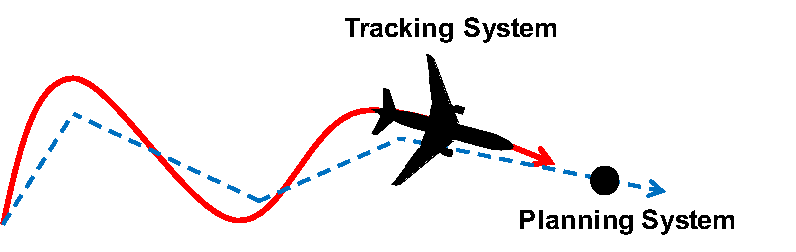
\includegraphics[width=0.35\textwidth]{fig/chasing}
	\caption{A planning system using a fast but simple model, followed by a tracking system using a dynamic model}
	\label{fig:chasing}
	\vspace{-.2in}
\end{figure}
%
Because we designed FaSTrackHD to be modular, it can be used with most existing fast path or trajectory planners, enabling motion planning that is rapid, safe, and dynamically accurate. In this paper, we demonstrate this tool by computing the tracking error bound between a 10D quadrotor model affected by wind and a linear 3D kinematic model. Online, the simulated system travels through a static, windy environment with obstacles that are only known once they are within the limited sensing range of the vehicle. Combining this bound with a kinematic rapidly exploring random trees (RRT) fast path planner, the system is able to safely plan and track a trajectory through the environment in real time.